%
% flugzeugachsen.tex -- Flugzeugachsen und Drehbewegungen
%
% (c) 2026 OST Ostschweizer Fachhochschule
%
\documentclass[tikz]{standalone}
\usepackage{amsmath}
\usepackage{times}
\usepackage{txfonts}
\usepackage{graphicx}
\usetikzlibrary{arrows,calc}
\definecolor{darkred}{rgb}{0.8,0,0}
\definecolor{darkgreen}{rgb}{0,0.6,0}
\begin{document}
\begin{tikzpicture}[>=latex]
% Bild ohne Text, Breite = Satzspiegel des Buches (126mm) -> Schrift bleibt 10pt
\node[anchor=south west,inner sep=0] (bild) at (0,0)
	{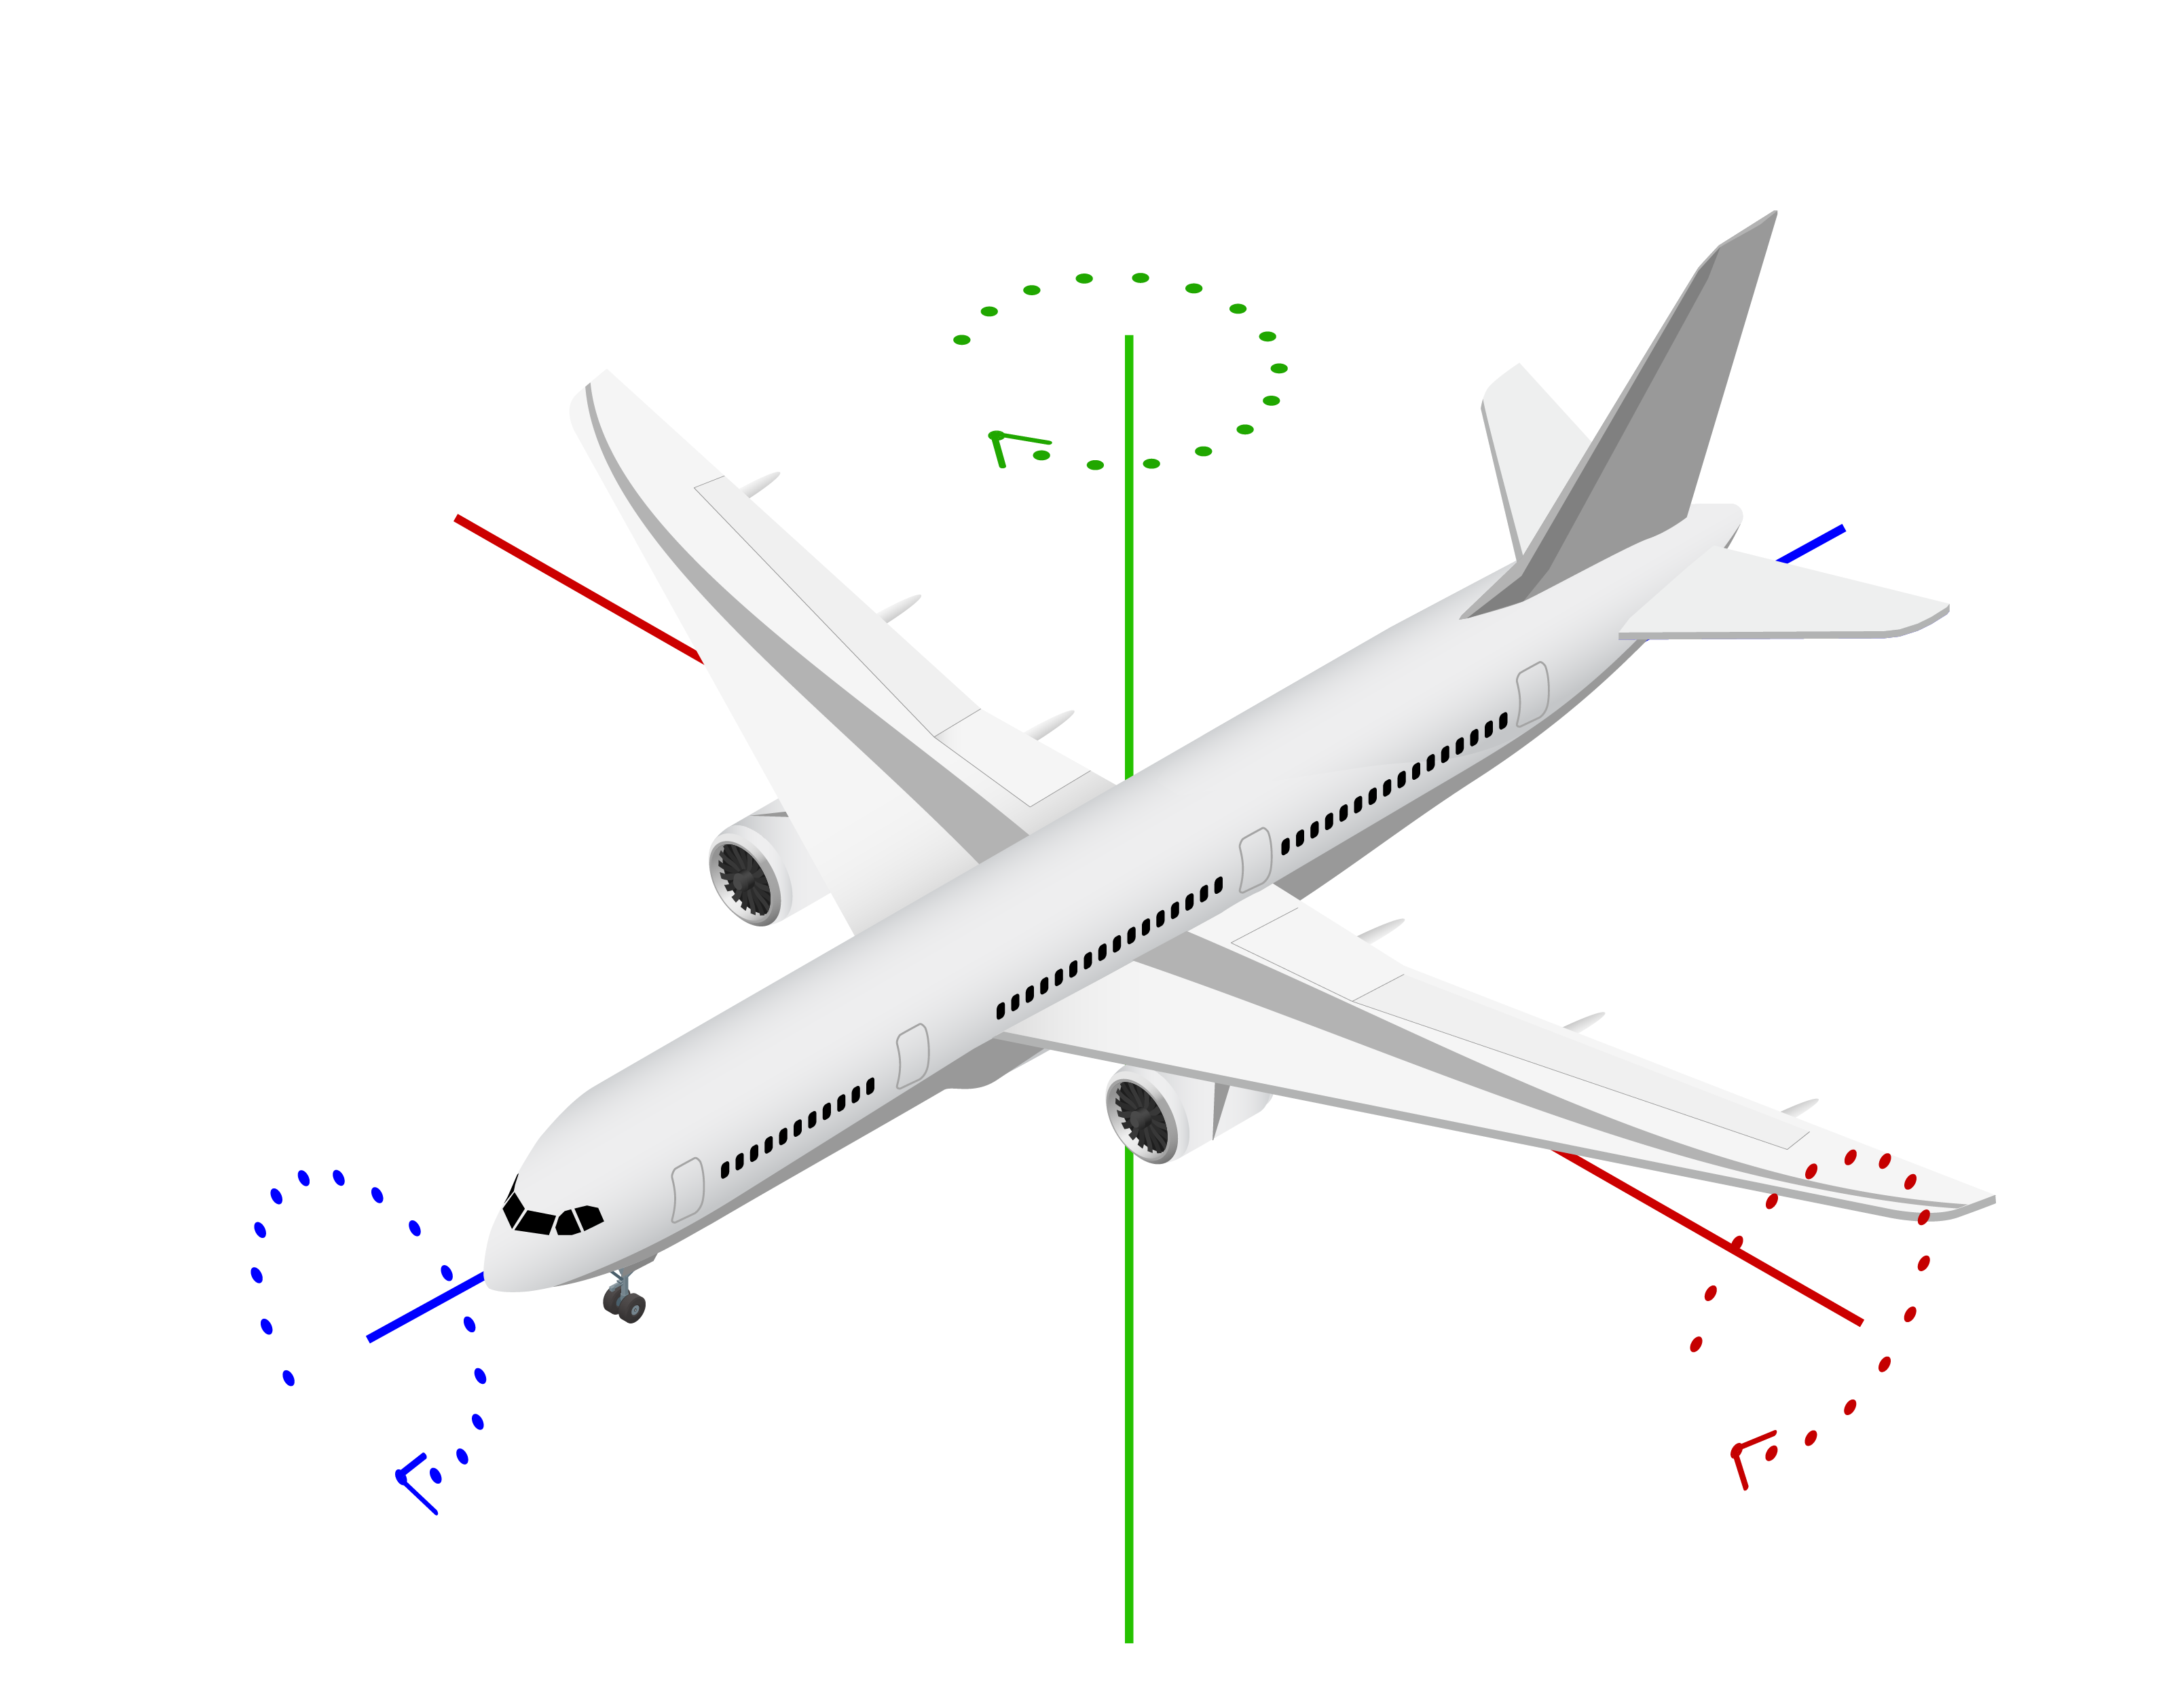
\includegraphics[width=10cm]{flugzeugachsen.png}};
\begin{scope}[x={(bild.south east)},y={(bild.north west)}]
	% Hochachse (gruen), oben
	\node[align=center] at (0.51,1.01)
		{\textcolor{darkgreen}{Gieren (Yaw)}\\Hochachse (Vertical Axis)};
	% Laengsachse (blau), unten links
	\node[align=center,anchor=west] at (0.04,-0.05)
		{\textcolor{blue}{Rollen (Roll)}\\Längsachse\\(Longitudinal Axis)};
	% Querachse (rot), unten rechts
	\node[align=center,anchor=east] at (0.98,-0.05)
		{\textcolor{darkred}{Nicken (Pitch)}\\Querachse\\(Lateral Axis)};
\end{scope}
\end{tikzpicture}
\end{document}
